\documentclass[12pt,a4paper]{article}

\usepackage[utf8]{inputenc}
\usepackage[T1]{fontenc}
\usepackage{graphicx}
\usepackage{booktabs}
\usepackage{amsmath}
\usepackage{hyperref}
\usepackage{geometry}
\usepackage{caption}
\usepackage{float}
\usepackage{array}

\geometry{margin=2.5cm}

\title{\textbf{Facial Expression Recognition System} \\[4pt]
\large A Deep Learning Approach Using Convolutional Neural Networks}
\author{Project Report}
\date{\today}

\begin{document}

\maketitle
\thispagestyle{empty}
\newpage

\tableofcontents
\newpage

\section{Abstract}
This report documents the development of a Facial Expression Recognition (FER) system capable of classifying seven distinct human emotions---angry, disgust, fear, happy, neutral, sad, and surprise---from facial images. The system is built using a custom Convolutional Neural Network (CNN) implemented with TensorFlow and Keras. It encompasses a complete pipeline spanning data preprocessing, model training with GPU acceleration, offline evaluation, and real-time webcam-based inference. The final model achieves a test accuracy of 57\% on the FER2013-derived dataset and runs in real time using DirectML-accelerated inference on a local GPU.

\section{Introduction}
Facial expression recognition is a fundamental problem in computer vision with applications in human-computer interaction, affective computing, mental health monitoring, and user experience analysis. The objective of this project was to build a complete FER system from scratch---from raw image data to a live webcam demo---using only TensorFlow and open-source computer vision libraries.

The system is organized into three interconnected modules:
\begin{enumerate}
    \item \textbf{Data Loading and Augmentation} --- Loads and preprocesses the dataset, applies on-the-fly augmentation for generalization.
    \item \textbf{Model Training} --- Defines, compiles, and trains a custom CNN with regularization techniques.
    \item \textbf{Evaluation and Real-Time Inference} --- Evaluates the model on a held-out test set and deploys it for live webcam-based emotion recognition.
\end{enumerate}

\section{Dataset Description}
The dataset used is derived from the FER2013 dataset, organized into a folder structure with two main directories:
\begin{itemize}
    \item \texttt{train/} --- Contains 22,968 grayscale images (48×48 pixels) across seven emotion classes.
    \item \texttt{test/} --- Contains 7,178 grayscale images (48×48 pixels) across the same seven emotion classes.
\end{itemize}

Each directory contains seven subfolders named after the emotion labels: \texttt{angry}, \texttt{disgust}, \texttt{fear}, \texttt{happy}, \texttt{neutral}, \texttt{sad}, and \texttt{surprise}.

\begin{table}[H]
    \centering
    \caption{Dataset distribution across emotion classes.}
    \label{tab:dataset}
    \begin{tabular}{lcc}
        \toprule
        Emotion & Train Samples & Test Samples \\
        \midrule
        Angry    & 3,995 & 958 \\
        Disgust  & 436   & 111 \\
        Fear     & 4,097 & 1,024 \\
        Happy    & 7,215 & 1,774 \\
        Neutral  & 4,965 & 1,233 \\
        Sad      & 4,830 & 1,247 \\
        Surprise & 3,171 & 831 \\
        \midrule
        Total    & 22,968 & 7,178 \\
        \bottomrule
    \end{tabular}
\end{table}

A notable characteristic is class imbalance: ``disgust'' has only 436 training samples versus 7,215 for ``happy''.

\section{Technical Approach}

\subsection{Data Loading and Augmentation (Part 1)}
The pipeline uses TensorFlow's \texttt{ImageDataGenerator} with \texttt{flow\_from\_directory}. This was chosen over \texttt{image\_dataset\_from\_directory} because it bundles augmentation and rescaling into the generator, producing objects that pass directly to \texttt{model.fit()} without extra preprocessing layers.

All images are loaded as grayscale and resized to 48×48 pixels. Training images receive on-the-fly augmentation: rotation up to $\pm 10^\circ$, zoom up to $\pm 10\%$, and random horizontal flips. Pixel values are normalized to $[0,1]$ by dividing by 255. A 20\% validation split is dynamically carved from the training folder. The test set receives only rescaling with no augmentation.

\subsection{Model Architecture (Part 2)}
The CNN follows a \texttt{Sequential} model with four convolutional blocks and a classification head. Each block consists of Conv2D (3×3, ReLU), BatchNormalization, MaxPooling2D (2×2), and Dropout. Filter counts double each block: 32 $\rightarrow$ 64 $\rightarrow$ 128 $\rightarrow$ 256. Dropout rates scale progressively from 0.25 to 0.50.

The classification head flattens the feature maps, passes them through a Dense(128, ReLU) layer with Dropout(0.5), and ends with a Dense(7, Softmax) output.

\begin{table}[H]
    \centering
    \caption{Model architecture summary.}
    \label{tab:architecture}
    \begin{tabular}{lc}
        \toprule
        Layer & Output Shape \\
        \midrule
        Conv2D + BN + MaxPool + Dropout(0.25) & (24, 24, 32) \\
        Conv2D + BN + MaxPool + Dropout(0.30) & (12, 12, 64) \\
        Conv2D + BN + MaxPool + Dropout(0.40) & (6, 6, 128) \\
        Conv2D + BN + MaxPool + Dropout(0.50) & (3, 3, 256) \\
        Flatten & (2304) \\
        Dense(128, ReLU) + Dropout(0.50) & (128) \\
        Dense(7, Softmax) & (7) \\
        \midrule
        Total parameters & 685,703 \\
        \bottomrule
    \end{tabular}
\end{table}

The model is compiled with Adam optimizer and categorical cross-entropy loss. Two callbacks are used: \texttt{ModelCheckpoint} saves the best weights as \texttt{emotion\_model.h5} based on validation loss; \texttt{EarlyStopping} with patience 10 halts training when validation loss plateaus and restores the best weights.

\subsection{GPU Acceleration}
Since TensorFlow $\geq$ 2.11 dropped native Windows GPU support, a Python 3.10 virtual environment was set up with TensorFlow 2.10.0 and Microsoft's \texttt{tensorflow-directml-plugin}. This enables GPU acceleration on any DirectX 12-compatible hardware. The system detected an NVIDIA Quadro P1000 and an Intel UHD Graphics 630.

\subsection{Evaluation and Real-Time Inference (Part 3)}

\subsubsection*{Offline Evaluation}
The model is evaluated on the full test set (7,178 images). Predictions are aggregated and compared against ground-truth labels to produce a classification report and confusion matrix. Run the following command to generate these metrics:

\begin{verbatim}
.\.venv310\Scripts\python.exe evaluate_webcam.py --mode eval
\end{verbatim}

This saves \texttt{confusion\_matrix.png} and prints per-class precision, recall, and F1-score.

\subsubsection*{Real-Time Webcam Inference}
The webcam mode loads the model and captures frames from the default camera using OpenCV. For each frame, it converts to grayscale, detects faces using Haar Cascade (\texttt{haarcascade\_frontalface\_default.xml}), and for each detected face crops, resizes to 48×48, normalizes, and runs \texttt{model.predict()}. The predicted emotion and confidence are drawn on the frame with a bounding box. Press 'q' to exit.

\begin{figure}[H]
    \centering
    \includegraphics[width=0.45\textwidth]{screenshot_webcam.png}
    \caption{Real-time webcam inference showing detected face with emotion label and confidence. \textit{Replace with your own screenshot.}}
    \label{fig:webcam}
\end{figure}

\section{Results}
The model achieved an overall accuracy of \textbf{57\%} on the test set. Run the evaluation command above to generate the confusion matrix and classification report on your machine. The most recent results are shown below.

\begin{table}[H]
    \centering
    \caption{Classification report on the test set.}
    \label{tab:results}
    \begin{tabular}{lcccc}
        \toprule
        Emotion & Precision & Recall & F1-Score & Support \\
        \midrule
        Angry    & 0.50 & 0.42 & 0.46 & 958 \\
        Disgust  & 0.00 & 0.00 & 0.00 & 111 \\
        Fear     & 0.43 & 0.11 & 0.17 & 1,024 \\
        Happy    & 0.80 & 0.83 & 0.81 & 1,774 \\
        Neutral  & 0.44 & 0.73 & 0.55 & 1,233 \\
        Sad      & 0.45 & 0.47 & 0.46 & 1,247 \\
        Surprise & 0.68 & 0.76 & 0.72 & 831 \\
        \midrule
        Accuracy & \multicolumn{3}{c}{0.57} & 7,178 \\
        \bottomrule
    \end{tabular}
\end{table}

\begin{figure}[H]
    \centering
    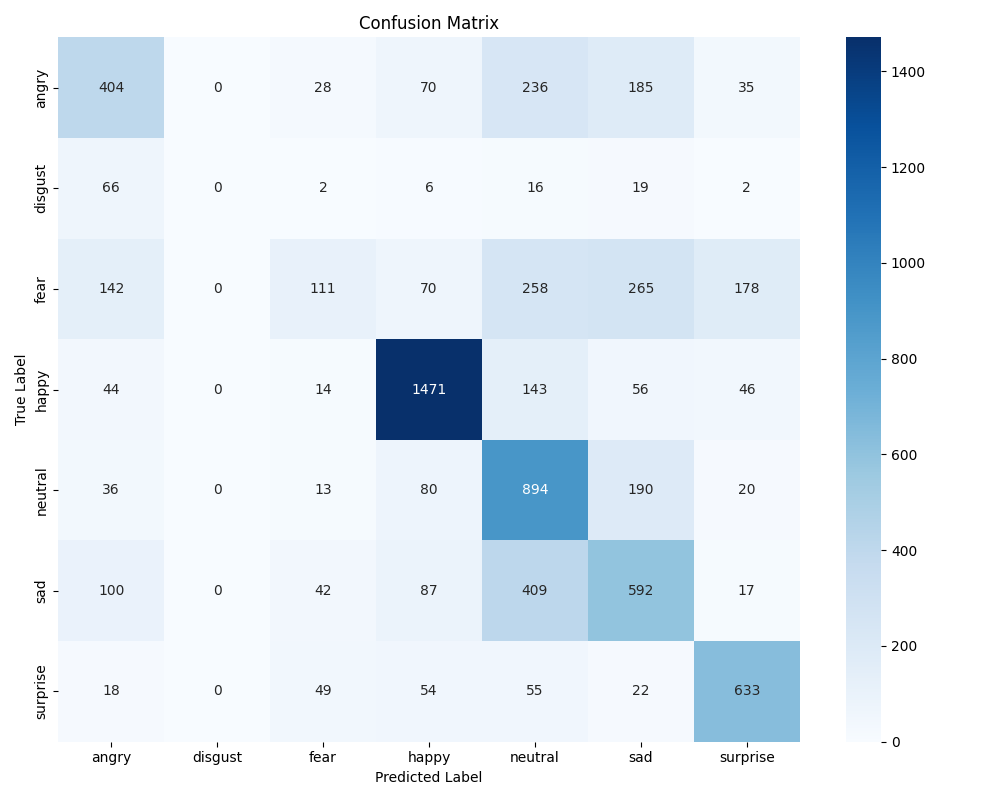
\includegraphics[width=0.85\textwidth]{confusion_matrix.png}
    \caption{Confusion matrix showing per-class prediction distribution on the test set. Generated by running the evaluation command.}
    \label{fig:confmat}
\end{figure}

\subsection{Analysis}
\textbf{Happy (F1 = 0.81)} performs best due to distinctive features and large sample size. \textbf{Surprise (F1 = 0.72)} also performs well with its characteristic raised eyebrows and open mouth. \textbf{Neutral (F1 = 0.55)} is moderate, often confused with sadness and anger. \textbf{Angry and Sad (F1 = 0.46)} share overlapping features like furrowed brows. \textbf{Fear (F1 = 0.17)} is frequently misclassified as surprise, sad, or neutral. \textbf{Disgust (F1 = 0.00)} is never predicted due to extreme class imbalance (only 111 test samples).

\section{Technical Choices}
Key decisions and their rationale:
\begin{itemize}
    \item \textbf{ImageDataGenerator} over \texttt{image\_dataset\_from\_directory} --- bundles augmentation + rescaling into one object; generators pass directly to \texttt{model.fit()}.
    \item \textbf{4 Conv blocks (32$\rightarrow$256 filters)} --- balances 685K parameters against real-time inference speed.
    \item \textbf{BatchNormalization + progressive dropout} --- stabilizes training and prevents overfitting on a 22K-sample dataset.
    \item \textbf{Adam optimizer} --- adaptive learning rate works well with noisy augmented data.
    \item \textbf{EarlyStopping (patience=10)} --- stops training when validation loss plateaus, saving time.
    \item \textbf{DirectML plugin} --- only viable GPU option on Windows for TF $\geq$ 2.11; works with any DirectX 12 GPU.
    \item \textbf{Haar Cascade} --- lightweight face detector; runs on CPU without GPU overhead.
    \item \textbf{Grayscale} --- FER2013 dataset is grayscale; emotion features are texture-based, not color-based.
\end{itemize}

\section{Project Files}
\begin{table}[H]
    \centering
    \caption{Project file structure.}
    \label{tab:files}
    \begin{tabular}{ll}
        \toprule
        File & Purpose \\
        \midrule
        \texttt{data\_loader.py} & Data loading, augmentation, and generator creation \\
        \texttt{model\_train.py} & CNN architecture, compilation, and training \\
        \texttt{evaluate\_webcam.py} & Offline evaluation and real-time webcam inference \\
        \texttt{emotion\_model.h5} & Trained model weights (best checkpoint) \\
        \texttt{confusion\_matrix.png} & Visual confusion matrix generated by eval mode \\
        \texttt{report.tex} & This LaTeX report \\
        \texttt{dataset/} & Image dataset (train/ and test/ subdirectories) \\
        \bottomrule
    \end{tabular}
\end{table}

\section{Conclusion}
This project successfully implemented a complete facial expression recognition pipeline from data loading to real-time deployment. The custom CNN with 685K parameters achieved 57\% accuracy on seven-class emotion classification, with ``happy'' and ``surprise'' being the most reliably detected emotions. The system runs in real time on consumer GPU hardware via DirectML acceleration.

\subsection*{Future Work}
\begin{itemize}
    \item Address class imbalance for ``disgust'' via oversampling or weighted loss functions.
    \item Explore deeper architectures (ResNet, EfficientNet) for improved accuracy.
    \item Replace Haar Cascade with a deep learning face detector (MTCNN, RetinaFace) for better detection of non-frontal faces.
    \item Fine-tune on in-the-wild data for better real-world generalization.
\end{itemize}

\end{document}
